\documentclass[]{article}

\usepackage[utf8]{inputenc}
\usepackage[paperheight=0.3in,paperwidth=1in,margin=.1mm]{geometry}
\usepackage{tikz}
\usetikzlibrary{shapes, arrows, calc}
\usepackage{color}

\usepackage{booktabs}  % nicer table borders 

\begin{document}

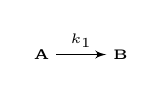
\begin{tikzpicture}[>=latex']
\tiny
\node  at (0, 0) (A) {$\bf A$};
\node  at (1, 0) (B) {$\bf B$};
\path (A) edge[->] node[above]{$k_1$} (B);
\end{tikzpicture} 
\end{document}

